\documentclass[12pt]{article}
\usepackage{amsmath}
\usepackage{fancyhdr}
\usepackage{geometry}
\usepackage{parskip}
\usepackage{pdfpages}
\usepackage{graphicx}
\graphicspath{{./}}
\geometry{letterpaper, portrait, margin=1in}
\setlength{\parindent}{0pt}

\title{Math 252 Homework\\
\large Sections 4.2 \& 4.3}
\date{2016/04/03}
\author{Solomon Greenberg}

\fancyhf{}
\pagestyle{fancy}

\lhead{Math 252 Homework --- Sections 4.2 \& 4.3 }
\rhead{Solomon Greenberg}



\begin{document}
    \pagenumbering{gobble}
    \newpage
    \pagenumbering{arabic}

    \section*{Chapter 4.2}
    \paragraph*{1:\\}
        An absolute minimum is a point at the lowest value that a graph reaches over an interval that, if the interval is open, does not include the limits of the interval. A relative minimum is any point that has a lesser value than the the points directly to the left or right of it.

    \paragraph*{5:\\}
        Local minima: (2, 2), (5, 3) \\
        Local maxima: (4, 5) \\
        Absolute minima: (0, 2), (2, 2) \\
        Absolute maxima: (4, 5) \\

    \paragraph*{11:\\} 
        a:\\ 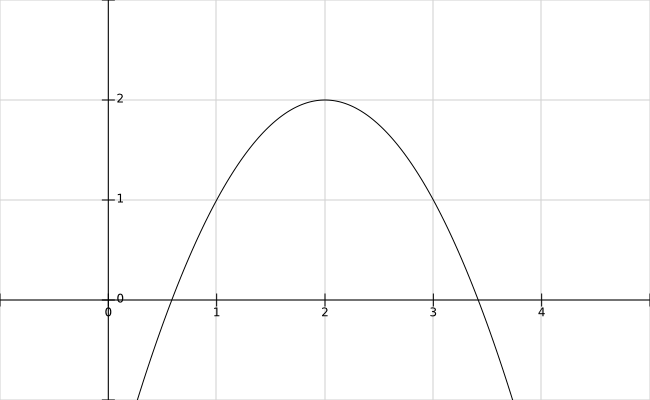
\includegraphics[scale=.333]{graph11a.png}\\\\
        b:\\ 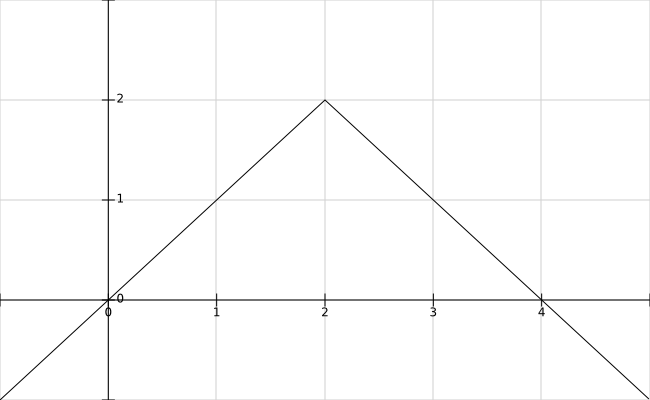
\includegraphics[scale=.333]{graph11b.png}\\\\
        c:\\ 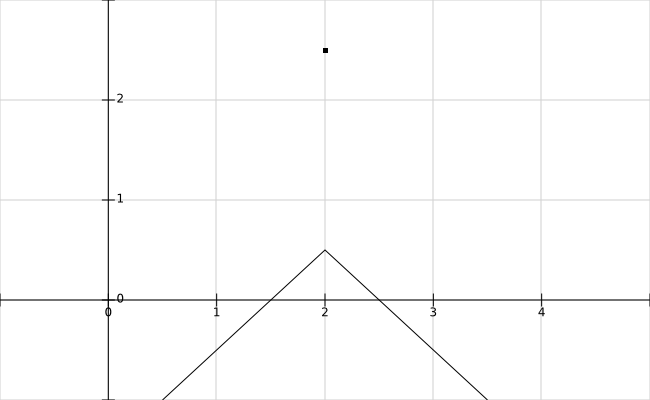
\includegraphics[scale=.333]{graph11c.png}\\\\

    \paragraph*{29:\\}
        Note: Used calculator (Ti-$n$spire CX CAS) to find x-intercepts of \begin {math} f'(y) \end {math} \\
        Critical numbers at \begin{math} x=\{0, 2\} \end {math}\\ 

    \paragraph*{35:\\}
        Note: used calculator (Ti-$n$spire CX CAS) to find x-intercepts of \begin{math} f'(\theta) \end{math} \\
        Critical numbers at \begin{math} \theta=\{2 \cdot n \cdot \pi, n \cdot \pi\} \end{math} \\

    \paragraph*{43:\\}
        Absolute maxima: $(-1, 8)$\\ Absolute minima: $(2, -18)$\\

    \paragraph*{51:\\}
        Absolute maxima: $(1, \ln(3))$\\ Absolute minima: $(1, \ln(1.75))$\\

    \paragraph*{59:\\}
        $f(x) = x\cdot \sqrt{x-x^2}$\\
        a: No absolute min/max as function is consistantly concave down and on an open interval.\\
        b: Likewise

    \paragraph*{61:\\}
        $V = 999.87 - 0.06426T - 0.0085043T^2 - 0.0000679T^3$\\
        Max.\ density at $x = 208.614$
    
    \section*{Chapter 4.3}
    \paragraph*{2:\\}
            Concave upward:   $(2, 4), (\frac{16}{3}, 8)$\\
            Concave downward: $(0, 2), (4, \frac{16}{3})$\\

    \paragraph*{6:\\}
        a: $(2, 4), (6, 9)$ --- if $f'(x)$ is positive, $x$ is increasing. \\
        b: $x = {0, 2, 4, 6}$ --- if $f'(x) = 0$, $f(x)$ is at a local max or min\\
        c: $(1, 3), (5, 7), (8, 9)$ --- if $f''(x) > 0$, $f(x)$ is concave up, and vice versa\\
        d: $x = {1, 3, 5, 7, 8, 9}$ --- inflection points are where $f''(x)$ changes from $<0$ to $>0$ or vice versa.\\
    
    \paragraph*{7:\\}
            a: Increase: $(-\infty, -3), (2, \infty)$\\
               Decrease: $(-3, 2)$\\
            b: Local max: $x = -3$\\Local min: $x = 2$ \\
            c: Concave down: $(-\infty, 0)$\\ Concave up: $(0, \infty)$\\
    
    \paragraph*{13:\\}
            a: Decreasing: $(-\infty, -\frac{\ln(2)}{3})$\\Increasing: $(-\frac{\ln(2)}{3}, \infty)$\\
            b: Local min: $x = -\frac{\ln(2)}{3}$\\
            c: Concave up: $(-\infty, \infty)$\\

    \paragraph*{20:\\}
            a: $x = {0, \frac{4}{7}, 1}$\\
            b: Determines whether the points are a relative maximum or minimum or other.\\
            $f''(0) = 0$, meaning $f(0)$ is an inflection point\\
            $f''(\frac{4}{7}) > 0$, meaning $f(\frac{4}{7})$ is a relative min\\
            $f''(1) = 0$, meaning $f(1)$ is an inflection point\\
            c: Tells whether a point is a relative min, relative max, or inflection point by taking values from either side of the critical point

    \paragraph*{23:\\}
            a: Increase: $(-\infty, -1), (0, 1)$\\Decrease: $(-1, 0), (1, \infty)$\\
            b: Local max: $x = {-1, 1}$\\Local min: $x = {0}$\\
            c: Concave down: $(-\infty, -\frac{\sqrt{3}}{3}), (\frac{\sqrt{3}}{3}, \infty)$\\
            Concave up: $(-\frac{\sqrt{3}}{3}, \frac{\sqrt{3}}{3})$\\
            d:\\ 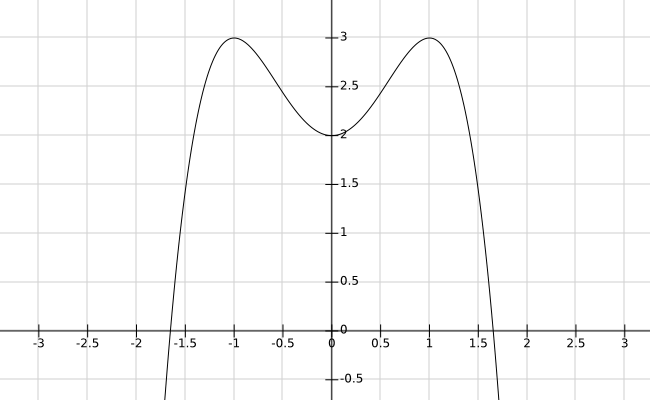
\includegraphics[scale=.333]{23.png}\\\\

    \paragraph*{30:\\}
            a: Increase: $(0, \infty)$\\Decrease: $(-\infty, 0)$\\
            b: Local min: $x = 3\cdot\ln(3)$\\
            c: Concave down: $(-\infty, 3), (3, \infty)$\\Concave up: $(3, 0), (0, 3)$\\
            Inflection points: $x = 3\cdot\ln(3)$\\

    \paragraph*{49:\\}
                Assuming I'm a standard well-tuned PD (Proportional-Derivitive) controller:\\
            a: Turn down thermostat\\
            b: Turn up a bit\\
            c: Turn down a bit \\
            d: Turn up\\
\thispagestyle{fancy}

\end{document}

